
%(BEGIN_QUESTION)
% Copyright 2015, Tony R. Kuphaldt, released under the Creative Commons Attribution License (v 1.0)
% This means you may do almost anything with this work of mine, so long as you give me proper credit

Skisser ledninger som kobler disse multi-ratio CT-ene til de tre amperemetrene, og sett inn skruer i kortslutningsterminalblokkene etter behov, slik at du får CT-forhold 200:5 på hver fase:

$$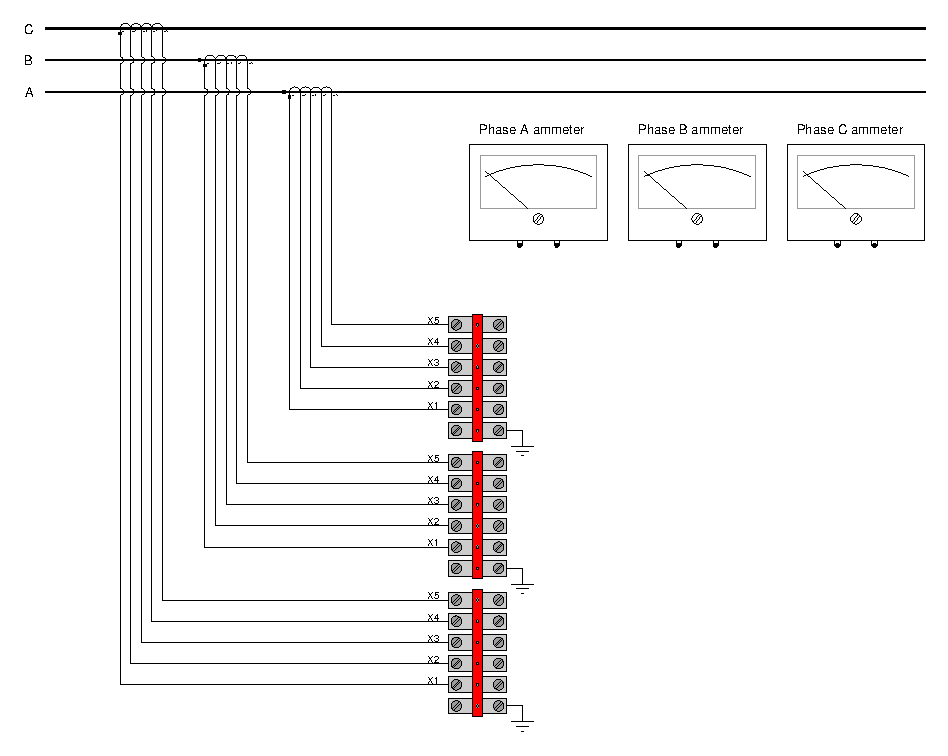
\includegraphics[width=15.5cm]{i01029x01.eps}$$

Anta at hver multi-ratio CT har følgende vindingstall mellom terminalpar:

\begin{itemize}
\item{} 10 vindinger mellom X1 og X2
\item{} 5 vindinger mellom X2 og X3
\item{} 25 vindinger mellom X3 og X4
\item{} 20 vindinger mellom X4 og X5
\end{itemize}


\vfil 

\underbar{file i01029}
\eject
%(END_QUESTION)





%(BEGIN_ANSWER)

Dette er en vurderingsoppgave -- ingen fasit eller hint oppgis!
 
%(END_ANSWER)





%(BEGIN_NOTES)

Ønsket forhold 200:5 tilsvarer 40:1. Da må terminalparet gi totalt 40 vindinger: X1-X4 (10+5+25). To jordingsskruer settes i hver kortslutningsterminalblokk: én for kortslutningsbøylen til jord, og én for å jorde én CT-sekundærterminal (typisk høyere terminalnummer, her X4).

$$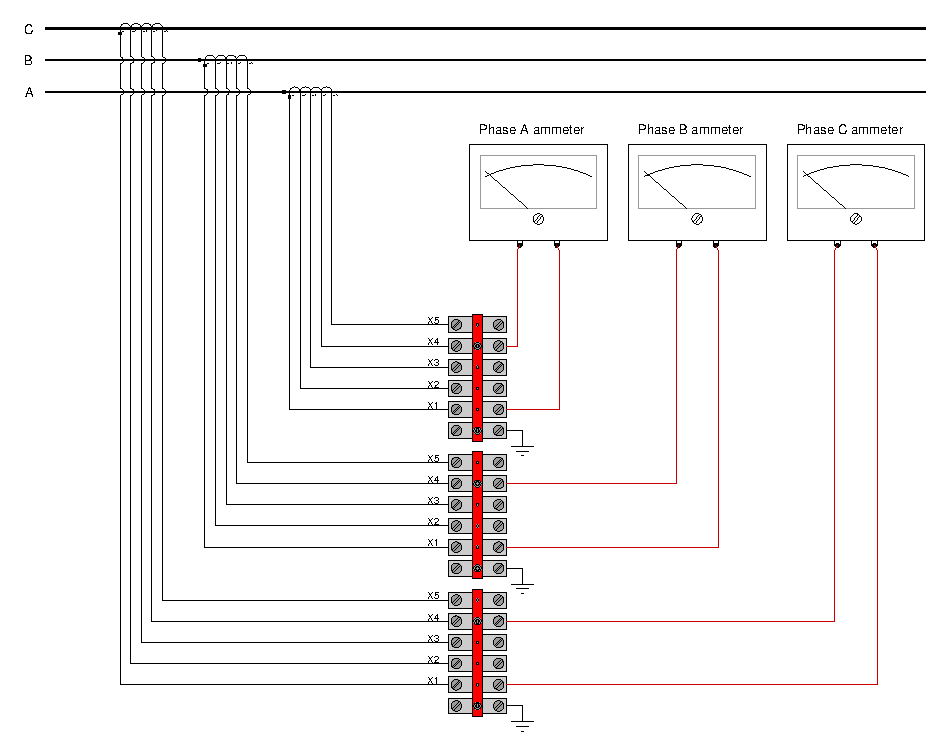
\includegraphics[width=15.5cm]{i01029x02.eps}$$

%INDEX% Protective relay: shorting terminal block

%(END_NOTES)

